
One fundamental part of all software development is the concept of
abstraction. Abstraction can be described as a way of decomposing  an
application into different levels, with different level of detail. This
allows us to forget about certain details of the software, and  instead
focus on other details. Consider the development of a simple game with
basic 2D graphics. On a very low level, this requires a tremendous
amount of work in order to shuffle data between hardware buses, perform
memory accesses and CPU operations. By using higher abstraction levels,
we can let third-party frameworks take care of stuff such as drawing
graphics to the screen, let the operating system and programming
language take care of bus and memory accesses. This allows us to focus
on designing the game logic itself, and just forget all about the
necessary stuff that just works.\cite{paper:abstraction}\\

In the same way, testing can be performed at several different levels.
There are several ways of defining these levels, but one way of
describing it is like a pyramid (\fref{fig:testing_pyramid}). We can
imagine testing at different levels as holding a flashlight at different
levels of the pyramid. If we hold the flashlight at the top of the
pyramid, the flashlight will illuminate a large part of the pyramid. If
the flashlight is hold at the bottom of the pyramid, a much smaller
piece of the pyramid will be illuminated. Similar to this, testing at a
high level lets us forget about a lot of details, and a large part of
the code must be run in order for the test to complete. Testing at a
lower level requires a much smaller part of the code to be run.
Different levels of testing has different advantages, drawbacks and
uses, which will be covered in the following subsections.\\

\begin{figure}
\centering
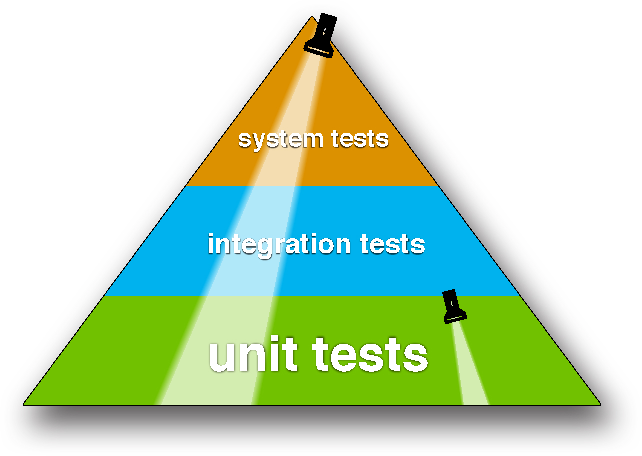
\includegraphics[width=0.7\textwidth]{theory/levels/triangle}
\caption{The software testing pyramid, with two flashlights at different
         levels illustrating how the level of testing affects the amount
         of tested code.}
\label{fig:testing_pyramid}
\end{figure}
